% EVALID methodology paper -- arXiv source
% Compile: pdflatex main && bibtex main && pdflatex main && pdflatex main
%
\documentclass[11pt,a4paper]{article}

\usepackage[T1]{fontenc}
\usepackage[utf8]{inputenc}
\usepackage{lmodern}
\usepackage{amsmath,amssymb}
\usepackage{booktabs}
\usepackage{graphicx}
\usepackage{microtype}
\usepackage[margin=1in]{geometry}
\usepackage[hidelinks]{hyperref}
\usepackage{orcidlink}
\usepackage{xcolor}

\newcommand{\todo}[1]{\textcolor{red}{\textbf{[TODO: #1]}}}
\newcommand{\verdict}[1]{\textsc{#1}}

\title{EVALID: A Pre-Registered Identifiability Protocol for Bounding
Nuisance Capacity in Empirical Claims}

\author{Lukas A. Sosna\,\orcidlink{0009-0004-1266-9729}\\
\small Independent Researcher\\
\small \texttt{ORCID: 0009-0004-1266-9729}}

\date{\today}

\begin{document}
\maketitle

\begin{abstract}
A claim that a system possesses a capability, evidenced by a score on an
instrument, can fail in four distinct places: the instrument may carry a
channel that produces the score without the capability; the estimator may be
degenerate with nuisance parameters, so the score is unattributable even if the
capability is real; the analysis may contain multiplicity, unit or arithmetic
errors; or the claim may have been selected after seeing the data. We present
EVALID, a pre-registered audit protocol that addresses all four by fixing
predictions, numeric thresholds and the resampling unit in writing before data
are loaded, publishing passes and failures alike, and logging every correction
rather than repairing it silently. EVALID does not certify that a capability is
real; it bounds how much of a reported quantity can be produced without it, and
reports whether the remainder is identifiable, via a closed verdict lattice.
We report a worked example in which the protocol was aimed at the present
author's own prior gravitational-wave dispersion proposal: twelve of thirteen
registered predictions fail, three of them fatally and independently. We
further report that the protocol caught a defect in that audit's own output --
a threshold comparison of $0.952$ against a registered threshold of $0.95$
whose value moved by up to $0.096$ under a change of numerical implementation
alone -- and that closing this defect required a change to the protocol itself.
We argue that the number of published corrections, and the fraction of them
found by someone other than the author, are the appropriate quality metrics for
an audit programme.
\end{abstract}

\section{Introduction}
\label{sec:intro}

\subsection{The problem}

Reported scores are load-bearing. A benchmark number decides which model ships;
a fitted coefficient decides which theory is pursued. In both cases the
inference runs from a measured quantity $X$ to a claimed property $C$, and in
both cases that inference can be broken without anyone being dishonest.

Four failure modes matter, and they are independent:

\begin{enumerate}
\item \textbf{Instrument channel.} $X$ is partly produced by structure in the
instrument that has nothing to do with $C$. Question-blind accuracy above
chance on a multiple-choice benchmark is an instance
\cite{balepur2024artifacts}.
\item \textbf{Estimator degeneracy.} The parameter carrying $C$ is not
separable from nuisance parameters, so $X$ cannot be attributed to $C$ even
where $C$ exists. This is an identifiability failure, not a power failure, and
more data does not fix it \cite{vallisneri2008fisher}.
\item \textbf{Analysis error.} Multiplicity uncontrolled, resampling unit
inconsistent between an interval and its $p$-value, arithmetic wrong.
\item \textbf{Selection.} The tested prediction was chosen after the data were
seen.
\end{enumerate}

Existing practice addresses these piecemeal. Pre-registration is standard in
clinical trials and increasingly in psychology, but rare in machine-learning
evaluation and in exploratory astrophysics. Identifiability analysis is
standard in gravitational-wave parameter estimation and rare elsewhere.
Multiplicity control is standard in genomics. No single convention requires all
four at once, and the failure modes compound: an instrument channel that is
also degenerate with a nuisance parameter is invisible to any test that
addresses only one.

\subsection{Contribution}

We do not claim novelty for any individual component. Pre-registration,
Benjamini--Hochberg control \cite{benjamini1995controlling}, cluster bootstrap
resampling, Fisher-matrix identifiability analysis
\cite{cutler1994gravitational} and question-blind probing
\cite{balepur2024artifacts} are all prior art. Where we report question-blind
results, the method is Balepur et al.'s, not ours.

Our contribution is the \emph{audit framing}: a protocol that composes these
into a pre-registered procedure with a closed verdict lattice, mandatory
numerical uncertainty on every threshold comparison, and a published correction
log; and evidence that the composition catches failures the components do not
catch individually, including in the protocol's own output.

\subsection{Disclosure}
\label{sec:disclosure}

The gravitational-wave framework audited in \S\ref{sec:gw} is the present
author's own prior work. We wrote the theory, then wrote the protocol, then
aimed the protocol at the theory. Protocol \S7 makes this disclosure mandatory
and it is stated here rather than in a footnote.

We regard this as the strongest available evidence about the protocol rather
than a limitation of it. A procedure for bounding evidence that cannot demolish
its author's own theory gives no reason to believe it will demolish anyone
else's.

\section{The protocol}
\label{sec:protocol}

\subsection{Pre-registration}

Before data are loaded, a document fixes: the object of audit and its author;
whether the auditor and that author are the same person; numbered predictions
each with a numeric pass and fail condition; the resampling unit; the
multiplicity family and level; the sidedness of every test; and a deviations
policy. The document is hashed into the release manifest and is not edited
afterwards. Predictions later found to be invalid are retained and marked
\verdict{registered\_invalid}, never deleted.

Two requirements deserve emphasis because both were violated in our own work
before they were written down.

\paragraph{Unit consistency.} Every interval and every $p$-value for a given
quantity must use the declared resampling unit. Choosing a clustered confidence 
interval and an unclustered $p$-value for the same quantity is a protocol violation, 
not a modelling choice. In a concurrent benchmark audit (correction log and
corrigendum in the accompanying repository), this single inconsistency moved a headline $p$-value from $6\times10^{-10}$ to $0.0405$ and
cost the finding its multiplicity survival.

\paragraph{Sidedness.} A one-sided screen cannot observe effects that run
backwards. In the aforementioned benchmark audit, the per-subject screen was one-sided 
and the report never said so; a two-sided procedure detects a subject at $13.64\%$
question-blind accuracy on $n=110$ --- significantly \emph{anti}-predicted,
meaning the instrument channel exists there but runs in reverse.

\subsection{The verdict lattice}

The lattice is closed; an audit may not emit a verdict outside it. Per
prediction: \verdict{pass}, \verdict{fail}, \verdict{indeterminate},
\verdict{underdetermined}, \verdict{registered\_invalid}, \verdict{not\_run}.
Terminal: \verdict{identified}, \verdict{detected-but-not-identified},
\verdict{localized}, \verdict{none}, \verdict{artifact}.

A null is reported with its detection limit --- the smallest effect the
registered configuration would have detected --- and never as a proof of zero.

\subsection{Threshold comparison with mandatory uncertainty}
\label{sec:threshold}

This is the central methodological requirement and the one added in version
0.3.2:

\begin{quote}
Every quantity compared against a registered threshold ships with a numerical
uncertainty $u$, and a verdict inside that band is \verdict{indeterminate}.
\end{quote}

$u$ is estimated by grid refinement, finite-difference step variation, cluster
resampling, or --- required for any quantity involving a projection, an
orthogonalisation or a matrix inverse --- by computing it with at least two
independent implementations and taking the half-range.

The motivation is empirical and is given in \S\ref{sec:selfdefect}.

\subsection{Numerical admissibility}

Before any quantity derived from a matrix inverse is read, the condition number
is tested against a ceiling registered in advance; a matrix past the ceiling
yields \verdict{underdetermined} and its derived quantities are not reported.
Registering the ceiling in advance is what distinguishes this from discarding
an inconvenient result.

\subsection{Anchors and the correction log}

Every number printed in a report appears in an anchors file as a
claimed/recomputed pair bound to the file and location it was read from.
Coverage is reported as \emph{verified/defined}. Reporting ``29/29 passed''
from a file holding 38 entries is a true sentence that creates a false
impression, and an earlier version of our own protocol output published exactly that sentence.

Corrections are logged, never silently repaired, with the finder named.

\section{Worked example: falsifying the author's own theory}
\label{sec:gw}

\subsection{The object of audit}

The SRAG/SRLG framework proposes a logarithmic gravitational-wave dispersion,
\begin{equation}
\delta\Phi(\omega) = \frac{\lambda \ln(\omega_0/\omega)}{C(\lambda)},
\qquad C(\lambda) = 1 - e^{-\kappa|\lambda|^\beta},
\end{equation}
with $\kappa \approx 2.3$, $\beta \approx 1.2$ fitted to galactic rotation
curves. In observable form the waveform phase becomes
$\Psi(f) = \Psi_{\mathrm{GR}}(f) - A\ln(f/f_0)$ with $A \equiv \lambda/C(\lambda)$;
$f_0$ is absorbed exactly by the coalescence phase and is therefore not a
testable part of the hypothesis.

Thirteen predictions were registered with numeric thresholds before any
computation. Full pre-registration and report:
\texttt{audits/gw-srag/} in the accompanying repository.

\subsection{Results}

Twelve of thirteen predictions fail. Three are independently fatal.

\paragraph{The novelty claim is false.} A phase term $f^{\alpha-1}$ enters at
post-Newtonian order $n = (3\alpha+2)/2$. At $\alpha = 1$ the power-law
prefactor $1/(1-\alpha)$ diverges and the limit is exactly $\ln f$, at 2.5PN
--- where general relativity's own phase already carries a $\ln v$ term. The
proposed effect is a rescaling of a coefficient GR itself supplies, and
$\alpha = 1$ lies inside the tested set of the standard modified-dispersion
family \cite{mirshekari2012constraining, ligo2021tgr}.

\paragraph{It is not a propagation effect.} The stated formula contains no
distance. Distance scaling is the entire handle that makes the standard
dispersion test work, since the effect grows with propagation distance while
source-physics parameters do not \cite{mirshekari2012constraining}.

\paragraph{The effect is unobservable, not unobserved.} For a GW170817-like
binary neutron star ($\mathcal{M}_c = 1.188\,M_\odot$, $\eta = 0.2497$,
$\chi = 0$), TaylorF2 3.5PN aligned-spin \cite{buonanno2009comparison},
20--1610\,Hz, at fixed $\mathrm{SNR}=25$: $\sigma(A) = 0.0634$ with GR
parameters held fixed and $26.05$ once marginalised --- a degradation of
$410.9\times$, stable under parameter rescaling, grid refinement and
finite-difference step variation. A nonlinear check, which makes no
linearisation assumption, confirms it: a GR-only template recovers an injected
$1.06$\,rad coherent dephasing with fitting factor $0.99987$, leaving
$0.40\sigma$ of residual, absorbed by moving $\chi_{\mathrm{eff}}$ by $+0.0094$.

Because $C(\lambda) \to \kappa\lambda^\beta$ as $\lambda \to 0$, the amplitude
$A = \lambda/C(\lambda) \to \lambda^{-0.2}/\kappa$ \emph{diverges}, giving a
floor $\min_\lambda A = 0.7052$ at $\lambda^\star = 0.2103$. There is no value
of $\lambda$ for which the framework predicts a small effect.

\begin{table}[t]
\centering
\caption{Registered predictions and verdicts. Full evidence in the
accompanying repository; every number is anchored to its source file.}
\label{tab:gw}
\small
\begin{tabular}{llp{7.4cm}}
\toprule
ID & Verdict & Basis \\
\midrule
P1 & \verdict{fail} & $\alpha=1$ gives exactly $\ln f$ at 2.5PN; already constrained \\
P2a--e & \verdict{fail} & Five stated quantities not reproducible from the corpus's own formulas; the $\lambda$ table is inverted relative to its own definition \\
P3 & \verdict{fail} & Formula is distance-independent \\
P4 & \verdict{registered\_invalid} & Registered $1/\mathrm{SNR}$ criterion is wrong; superseded by P5 \\
P5 & \verdict{fail} & $|\rho|$ to $0.9992$; $\sigma(A)$ inflates $410.9\times$; $\mathrm{FF}=0.99987$ \\
P6 & \verdict{fail} & $\max_\alpha|\rho| = 0.99895$, threshold $0.95$ \\
P7 & \verdict{fail} & Exact $p = 0.0577$ at $r=0.5$, $n=15$; needs $n \geq 26$ \\
P8 & \verdict{fail} & Host path fraction $7.5\times10^{-5}$ to $5.0\times10^{-4}$ \\
P9 & \verdict{fail} & One confident multi-messenger event exists \\
\bottomrule
\end{tabular}
\end{table}

\section{The protocol catching a defect in its own output}
\label{sec:selfdefect}

Prediction P6 asked whether the logarithmic term is separable from the
power-law dispersion family, registering failure at
$\max_\alpha|\rho| \geq 0.95$ for the correlation between the $\ln f$ phase
basis and $f^{\alpha-1}$ after marginalising over
$\{\ln A, t_c, \phi_c, \ln\mathcal{M}_c, \ln\eta, \chi_{\mathrm{eff}}\}$.

The originally published table reported $\max|\rho| = 0.952$ and a profile
falling monotonically to $0.025$ at $\alpha = 4$. An independent re-run
recomputed the quantity four ways --- Gram--Schmidt projection with one pass
and with re-orthogonalisation, a Gram-matrix pseudo-inverse, and the
marginalised Fisher covariance, the last having no projector-implementation
freedom. All four agree to four decimal places, and none agrees with the
published table (Table~\ref{tab:p6}, Figure~\ref{fig:p6}).

\begin{table}[t]
\centering
\caption{Prediction P6 as published and as recomputed. The verdict direction is
unchanged; every value in the row was wrong, and the published figure was
materially misleading.}
\label{tab:p6}
\small
\begin{tabular}{lrrrr}
\toprule
$\alpha$ & Published & Recomputed & $\Delta$ & vs.\ threshold $0.95$ \\
\midrule
0   & 0.952 & \textbf{0.99895} & $+0.047$ & exceeds \\
0.5 & 0.900 & 0.94825 & $+0.048$ & $0.0018$ below \\
1.5 & 0.633 & \textbf{0.98170} & $+0.349$ & exceeds \\
2.5 & 0.285 & 0.91296 & $+0.628$ & below \\
3   & 0.139 & 0.86794 & $+0.729$ & below \\
3.5 & 0.036 & 0.81903 & $+0.783$ & below \\
4   & 0.025 & 0.76907 & $+0.744$ & below \\
\bottomrule
\end{tabular}
\end{table}

\begin{figure}[t]
\centering
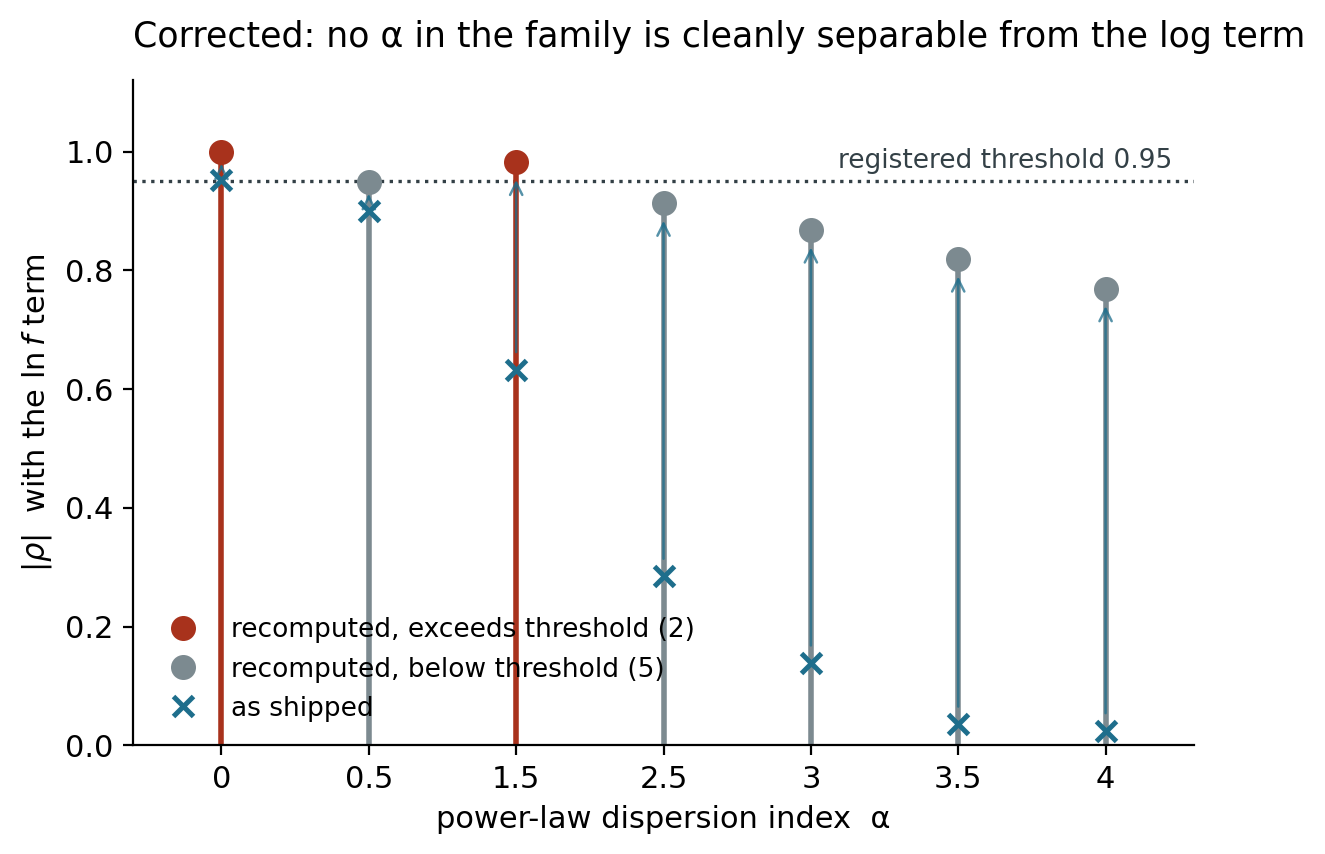
\includegraphics[width=0.78\textwidth]{figures/fig_p6_corrected.png}
\caption{Corrected P6. Circles are recomputed marginalised correlations;
crosses are the published values, with arrows showing the correction. Two
$\alpha$ values exceed the registered threshold and a third sits $0.0018$
below it; nothing in the family falls below $0.77$. The published figure showed
one value at the threshold and a clean monotone decay.}
\label{fig:p6}
\end{figure}

The methodological point is not the arithmetic. It is that the published
comparison was $0.952$ against $0.95$ --- a margin of $0.002$ --- with no
stated numerical uncertainty, while varying only the projection implementation
moved the same quantity by up to $0.096$, forty-eight times that margin. Under
the protocol as it then stood, a defensible-looking program could have returned
$0.948$ and reversed the verdict with no signal that anything was fragile.

A threshold comparison without a stated uncertainty is therefore undefined, and
\S\ref{sec:threshold} makes it a requirement. The protocol was revised by being
used against its author's work and failing.

\section{Discussion}
\label{sec:discussion}

\subsection{What EVALID does not do}

EVALID does not establish that a capability is real. A
\verdict{detected-but-not-identified} verdict says the excess is present and
unattributable, which is compatible with the capability existing. Nor does it
replace domain judgement: sidedness, unit consistency, disclosure and prior-art
attribution are decisions a program cannot make, and our conformance checker
says so explicitly rather than implying coverage it does not have.

\subsection{Correction rate as a quality metric}

Across three audits this programme has published fourteen corrections, eleven
found by someone other than the author. We propose that this ratio, rather than
the absence of corrections, is the appropriate quality signal for an audit
programme: an author whose published error rate is zero is an author who is not
being checked.

\section*{Data and code availability}

Protocol specification, library, the complete gravitational-wave audit with its
pre-registration, anchors, manifest and reproducer, and the correction log are
available at \url{https://github.com/LSosna/evalid} under the MIT licence, archived at
\url{https://doi.org/10.5281/zenodo.22545297}. The gravitational-wave audit is a forecast against published
constraints; no strain data were used. Reproduce with
\texttt{python audits/gw-srag/code/reproduce.py -{}-all}.

\section*{Competing interests}

The gravitational-wave framework audited in \S\ref{sec:gw} is the author's own
prior work; see \S\ref{sec:disclosure}. The author declares no financial
competing interests. This work was carried out independently, on the author's
own time and equipment, using publicly available data, and is not affiliated
with or funded by any institution.

\bibliographystyle{plainurl}
\bibliography{refs}

\end{document}
